% Codex--Overleaf local-replica sync probe: 2026-09-02 attempt 6
\documentclass[11pt]{article}

\usepackage[margin=1in]{geometry}
\usepackage{amsmath,booktabs,array}
\usepackage{graphicx}
\usepackage[hidelinks]{hyperref}
\usepackage{xcolor}
\usepackage{enumitem}
\usepackage{amsfonts}

\setlist[itemize]{leftmargin=1.5em,itemsep=0.25em,topsep=0.35em}
\setlist[enumerate]{leftmargin=1.8em,itemsep=0.25em,topsep=0.35em}
\newcommand{\code}[1]{\texttt{#1}}
\newcommand{\status}[1]{\textcolor{blue!65!black}{\textbf{#1}}}

\title{Racer-LLM Experiment Progress Log}
\author{}
\date{Last updated: September 1, 2026}

\begin{document}
\maketitle

\section{Project direction}

The main goal is to study the behavior and limitations of LLM-based policies in
a real-time multi-agent racing task. The baseline work is meant to provide
stable and understandable comparisons,instead of an exact
reproduction of every low-level detail in earlier racing systems of $\alpha$-racer or IBR from Wang et. al.. Should not diverge and get stuck in off-topic details, like tuning for better LLM agent performance.

The current comparison plans will eventually include:
\begin{itemize}
  \item locally trained and released $\alpha$-RACER policy;
  \item iterated best-response (IBR) policy;
  \item pure rule-based policy;
  \item LLM policy;
  \item LLM policy with explicit prompt rules.
\end{itemize}

The parameterized policies share the same local MPC and simulator wherever
possible. IBR is a separate online trajectory-optimization baseline and should
be described as such.

\section{August 10--12, 2026: local $\alpha$-RACER training}

\status{Status: implemented, trained, and provisionally validated.}

\subsection{$\alpha$-RACER in brief}

$\alpha$-RACER represents each car's high-level policy using five parameters
\[
  \theta_i=(q_i,\zeta_i,s_{1,i},s_{2,i},s_{3,i}).
\]
The parameters control how the MPC follows and modifies a precomputed
single-agent raceline, including tracking aggressiveness, speed along the
raceline, overtaking, and blocking behavior.

For a joint policy for three car $\theta=(\theta_0,\theta_1,\theta_2) \in \Theta^3$, car $i$ has a
long-term value
\[
  V_i(x,\theta)=\mathbb E\left[\sum_t\gamma^t r^i_t\right].
\]
In the paper they use artificial neuron network $\Phi$ to learn from generated racing records data and to approximate the changes of race state value respect to single agent variation:
\[
\begin{split}
  &\Phi(x,\theta'_i,\theta_{-i})-\Phi(x,\theta_i,\theta_{-i})\\
  &\qquad\approx
  V_i(x,\theta'_i,\theta_{-i})-V_i(x,\theta_i,\theta_{-i}).
\end{split}
\]
The function learned offline is later used in online policy searches for joint
parameters that give a high potential value and executes its own five-parameter
block.


\subsection{Local implementation}

The current implemented pipeline contains three
clearly separated stages.

\paragraph{1. Rollout collection.}
For each group, a baseline joint parameter set is sampled within the configured bounds of $(q,\zeta,s_1,s_2,s_3)$. Four races are simulated, resample the five control parameters of single agent:
\begin{enumerate}
  \item the baseline parameters for all three cars: $(\theta_0,\theta_1,\theta_2)$;
  \item a unilateral parameter change for car 0: $(\theta_0',\theta_1,\theta_2)$;
  \item a unilateral parameter change for car 1: $(\theta_0,\theta_1',\theta_2)$;
  \item a unilateral parameter change for car 2: $(\theta_0,\theta_1,\theta_2')$.
\end{enumerate}
Only one car's parameters change in each deviation race. This gives paired data
for learning the effect of unilateral policy changes.

At each control update, the code stores a 39-dimensional feature vector (relative progress, vehicle states, track curvature, and all 15 policy
parameters). The local single-step reward is currently the closing the gap or extending the lead against the fastest rivals, plus the safety term of off-road or collision penalty:
\[
  r^i_t=w_p\Delta s^i_t
  -w_o\mathbf{1}_{\mathrm{offroad},i}
  -w_c\mathbf{1}_{\mathrm{collision}}.
\]

The final feature data would be at the shape of ($N_{group}$, 4, time\_steps, 39). 4 represents 4 pairs of data per group and 39 represents the feature dimension as well as the size of the input for value function and potential function.

\paragraph{2. Value-function training.}
After a rollout finishes, discounted returns are computed backwards:
\[
  G^i_t=\sum_{k=t}^{T-1}\gamma^{k-t}r^i_k.
\]
And the value function $\widehat{V}_i(x,\theta)$ is trained using this Monte-Carlo learning to maximize the discounted accumulative returns $G_t$. The loss function:
\[
\mathcal{L}_{V_i}=\mathbf{MSE}(\widehat{V}_i(z_i),G^i_t)
\]

\paragraph{3. Potential-function training.}
The three trained value networks produce targets for unilateral value changes.
The potential network is trained so that
\[
  \widehat\Phi(x,\theta')-\widehat\Phi(x,\theta)
  \approx
  \widehat V_i(x,\theta')-\widehat V_i(x,\theta).
\]
Both sides are evaluated at the same baseline state. This avoids mixing a policy
change with the different state trajectory that the policy later causes.
The loss function:
\[
\mathcal{L}_{\Phi}=\mathbf{MSE}(\Delta \widehat V_i(x)-\Delta \widehat \Phi_i(x))
=
\frac{1}{\mathcal D_\Phi}\sum_{(x,\theta,\theta')}(\widehat V_i(x,\theta')-\widehat V_i(x,\theta),
\widehat\Phi(x,\theta')-\widehat\Phi(x,\theta))^2,
\]
Existing generated rollout data and trained checkpoints are reused automatically. If there is new rollout data the code would automatically re-train the later stage.

\subsection{Connection to the released code}

\begin{center}
\small
\begin{tabular}{p{0.20\linewidth}p{0.35\linewidth}p{0.35\linewidth}}
\toprule
Task & Released repository & Local project \\
\midrule
Collect races &
\code{collect\_data.bash}, \code{multi\_car\_blocking.py},
\code{merge\_data.py} &
\code{collect\_rollout\_data()} \\
Fit three values &
\code{train\_q\_model\_multi.py},
\code{train\_q\_model\_multi\_rel.py} &
\code{train\_value\_functions()} \\
Fit potential &
\code{train\_p\_model\_multi\_dist.py} &
\code{train\_potential\_function()} \\
Network definition &
\code{model\_arch.py::SimpleModel} &
\code{policy/alpha\_model.py::SimpleNeuralNetwork} \\
Online policy &
Released numerical simulator &
\code{policy/alpha\_racer.py::AlphaRacerPolicy} \\
\bottomrule
\end{tabular}
\end{center}

The local implementation keeps the original overall idea but exclude the ROS simulation dependency and change the chaining order of data pairs to more independent deviation groups of 4 shown previously.

\subsection{Training run recorded}

\begin{itemize}
  \item Track: Berlin.
  \item Vehicle model: local kinematic model.
  \item MPC horizon: 10.
  \item Data: 100 groups $\times$ 4 rollouts $\times$ 120 control samples.
  \item Rollout duration: 12 s.
  \item Discount: $\gamma=0.98$.
  \item Seed: 7.
  \item Value validation MSE: 21.43, 20.95, and 22.63.
  \item Best potential difference MSE: 0.0761.
\end{itemize}

\subsection{Initial three-position checkpoint comparison}

We make evaluation of locally trained weight using the standard three-position sweep on the Berlin track.
Each race(50s) contained three same $\alpha$-RACER cars.

\begin{center}
\small
\begin{tabular}{lcc}
\toprule
Checkpoint & Mean progress gain per car & Mean speed \\
\midrule
Released potential weights & 180.80 m & 3.56 m/s \\
Reimplementation trained & 198.64 m & 3.90 m/s \\
\bottomrule
\end{tabular} 
\end{center}

In shows that the locally trained checkpoint increased the mean
progress gain by 17.85 m and the mean speed by approximately 0.35 m/s. Neither configuration produced a recorded collision. The released checkpoint had no recorded off-road time, while the local checkpoint accumulated 0.08 seconds of off-road time across the nine vehicle trajectories.

These results show that the locally trained checkpoint runs successfully and
achieves higher progress under the local vehicle dynamics. It is therefore
suitable for use as the current $\alpha$-RACER baseline. 

\section{August 10--17, 2026: ordinary local IBR}

\status{Status: implemented and tested with SE disabled.}

The other thing we worked on was replacing the problematic IBR inherited from
the released $\alpha$-RACER code. The new version is based on the main idea in Wang et al.: iteratively update the planned trajectory against the opponent agent.

The current implementation does not copy Wang's low-level
solver but uses the state and controls already used in this project:
\[
  x_i=[s_i,e_i,\Delta\psi_i,v_i]^\top,
  \qquad
  u_i=[\text{throttle}_i,\text{steer}_i]^\top.
\]

Wang's ordinary IBR alternates best responses: one car optimizes its trajectory
while the other planned trajectories are fixed, and the updated plans are used
in the next round. Its racing objective mainly rewards progress, while vehicle
dynamics, track containment, and collision avoidance define the feasible
trajectories. We keep this general structure but use the local kinematic model
rather than Wang's trajectory parameterization and low-level solver.

\subsection{Local IBR best-response problem}

At each IBR update, the three-car interaction is reduced to a two-player
best-response problem between one car and its nearest longitudinal neighbour, which is identical to the IBR in the alpha-racer project.
During car $i$'s best response, the latest opponent trajectory
$\bar x_j=\{\bar s_{j,k},\bar e_{j,k}\}_{k=0}^{N}$ is held fixed. Car $i$
optimizes the Frenet state and normalized control sequences
\[
  x_{i,k}=
  \begin{bmatrix}
    s_{i,k} & e_{i,k} & \psi_{i,k}^{e} & v_{i,k}
  \end{bmatrix}^{\top},
  \qquad
  u_{i,k}=
  \begin{bmatrix}
    u_{i,k}^{a} & u_{i,k}^{\delta}
  \end{bmatrix}^{\top},
\]
where $s$ is unwrapped progress along the track centreline, $e$ is lateral
displacement from the centreline, $\psi^e$ is heading error, $v$ is speed, and
$u^a$ and $u^\delta$ are normalized throttle and steering commands.

The implemented best-response problem is
\[
\begin{aligned}
\min_{\substack{x_{i,0:N},\,u_{i,0:N-1},\\
                \epsilon^t_{i,1:N},\,\epsilon^c_{ij,1:N}}}
J_i
={}&
-w_p\bigl(s_{i,N}-s_{i,0}\bigr)
+w_e\sum_{k=0}^{N-1} e_{i,k}^{4} \\
&+w_{\Delta u}\sum_{k=0}^{N-1}
  \left\|u_{i,k}-u_{i,k-1}\right\|_2^2 \\
&+\rho_t\sum_{k=1}^{N}\left(\epsilon^t_{i,k}\right)^2
+\rho_c\sum_{k=1}^{N}\left(\epsilon^c_{ij,k}\right)^2 ,
\end{aligned}
\tag{1}
\]
subject to
\[
  x_{i,0}=x_i^{\mathrm{meas}},
\tag{2a}
\]
\[
  x_{i,k+1}=f_{\mathrm{F}}(x_{i,k},u_{i,k},\kappa_{i,k}),
  \qquad k=0,\ldots,N-1,
\tag{2b}
\]
\[
  -1\leq u_{i,k}^{a}\leq 1,
  \qquad
  -1\leq u_{i,k}^{\delta}\leq 1,
\tag{2c}
\]
\[
  0\leq v_{i,k+1}\leq v_{\max},
\tag{2d}
\]
\[
  \left|u_{i,k}^{\delta}-u_{i,k-1}^{\delta}\right|
  \leq \Delta u_{\max}^{\delta},
\tag{2e}
\]
\[
  \left|v_{i,k}^{2}\tan\!\left(u_{i,k}^{\delta}\right)\right|
  \leq \mu g L,
\tag{2f}
\]
\[
  |e_{i,k}|\leq e_{\max}+\epsilon^t_{i,k},
  \qquad
  \epsilon^t_{i,k}\geq0,
\tag{2g}
\]
and
\[
  \left(
    \frac{s_{i,k}-\bar s_{j,k}}{d_s}
  \right)^{p}
  +
  \left(
    \frac{e_{i,k}-\bar e_{j,k}}{d_e}
  \right)^{p}
  \geq
  1-\epsilon^c_{ij,k},
  \qquad
  \epsilon^c_{ij,k}\geq0.
\tag{2h}
\]
For $k=0$, the control-rate term and steering-rate constraint use the command
executed at the previous control update.

The discrete Frenet dynamics in (2b) are
\[
\begin{aligned}
s_{i,k+1}
&=s_{i,k}
+\Delta t\,
 \frac{v_{i,k}\cos\psi^e_{i,k}}
      {1-\kappa_{i,k}e_{i,k}},\\
e_{i,k+1}
&=e_{i,k}
+\Delta t\,v_{i,k}\sin\psi^e_{i,k},\\
\psi^e_{i,k+1}
&=\psi^e_{i,k}
+\Delta t\left[
  \frac{v_{i,k}}{L}\tan\delta_{i,k}
  -
  \frac{v_{i,k}\cos\psi^e_{i,k}\kappa_{i,k}}
       {1-\kappa_{i,k}e_{i,k}}
\right],\\
v_{i,k+1}
&=v_{i,k}
+\Delta t\,a_{\mathrm{lon}}(u^a_{i,k},v_{i,k}),
\end{aligned}
\tag{3}
\]
with
\[
  \delta_{i,k}=S_a u^\delta_{i,k}+S_b,
  \qquad
  L=L_F+L_R.
\]
The implementation replaces the Frenet denominator
$1-\kappa e$ by a smooth lower-bounded approximation near its singularity.
The longitudinal acceleration map $a_{\mathrm{lon}}$ is the same command model
used by the local simulator and MPC.

The first term of (1) rewards progress over the finite horizon. The $e^4$ term
penalizes centreline displacement weakly near $e=0$ but increasingly strongly
near the track boundary. The control-rate term discourages abrupt changes in
throttle and steering; unlike an earlier version, the retained objective has no
penalty on deviation from a locally chosen neutral command. The final two terms
penalize use of the track and collision slacks.

Constraint (2f) is the friction-based steering proxy shared with the local MPC.
It intentionally follows the released numerical implementation by applying
$\tan(\cdot)$ to the normalized steering command, whereas the state dynamics in
(3) use the physical steering angle
$\delta=S_a u^\delta+S_b$. Constraint (2g) softens the nominal track boundary.
Constraint (2h) is a differentiable and smooth superellipse separation(collision-avoidance) constraint;
physical contact in the simulator is checked separately using oriented vehicle
rectangles.

The current configuration uses
\[
\begin{gathered}
N=10,\qquad \Delta t=0.1~\mathrm{s},\qquad
w_p=10,\qquad w_e=10,\qquad w_{\Delta u}=0.10,\\
e_{\max}=0.44~\mathrm{m},\qquad
d_s=0.428~\mathrm{m},\qquad
d_e=0.285~\mathrm{m},\qquad p=4,\\
v_{\max}=5~\mathrm{m/s},\qquad
\Delta u_{\max}^{\delta}=0.4,\qquad
\mu=1.6,\qquad L=0.34~\mathrm{m}.
\end{gathered}
\]
The current shared-MPC defaults provide
$\rho_t=10^5$ and $\rho_c=10^4$. Both slacks remain enabled because the
hard-constraint ablations repeatedly became infeasible when initialized from
an already unsafe or closely packed state. Their activation and maximum values
are recorded in the experiment traces.

The solver also supports optional heading, speed-reference, and absolute-control
costs, but their current IBR weights are zero. In particular, the ordinary IBR
baseline uses the global $5~\mathrm{m/s}$ speed bound and does not track the
raceline speed profile. Its lateral objective is relative to the track
centreline rather than the optimized raceline.

A complete IBR round first solves car $i$'s best response to the opponent's
latest plan and then solves the opponent's best response to the updated plan.
The current implementation performs at most two such rounds, stops early when
the longitudinal/lateral plan change is below $10^{-3}$, and finally solves car
$i$ once more against the latest opponent plan. Only the first control of this
final plan is applied before the problem is rebuilt at the next control update.

The
fourth-power lateral term follows the form used by the released
$\alpha$-RACER IBR. It is small near the centre of the track but grows rapidly
near the boundary. The control-rate term is a standard local regularizer that
reduces abrupt command changes. We removed the earlier
$\|u-u_{\mathrm{neutral}}\|^2$ term because its neutral command was a local
design choice and was not needed by the tests.

It also shares the constraints with the local kinematic model and vehicle
parameters, uses normalized throttle and steering bounds, maximum speed,
steering-rate limit, and the same friction-based steering/speed limit used by
the local MPC. Track and collision constraints have explicit nonnegative slack
variables with large penalties. These are local feasibility devices rather
than part of Wang's original hard-constrained formulation, and their activation
is recorded.

\subsection{Objective and slack audit}

We selected the objective using six scenarios: the three Berlin starting
positions, a Berlin closing-speed case, and one case each on the Modena and
rounded-rectangle tracks. The table reports mean per-car progress gain and
aggregate event time over the six simulations.

\begin{table}[ht]
  \centering
  \small
  \begin{tabular}{lrrrr}
    \toprule
    IBR variant & Progress (m) & Off-road (s) & Collision (s) & Solver failure (s) \\
    \midrule
    Progress only & 82.24 & 11.42 & 1.58 & 0.10 \\
    $+\|\Delta u\|^2$ & 82.16 & 13.64 & 2.62 & 0.00 \\
    $+0.4e^2+\|\Delta u\|^2$ & 82.96 & 0.28 & 1.52 & 0.00 \\
    $+10e^4+\|\Delta u\|^2$ & 82.84 & 0.00 & 1.36 & 0.00 \\
    $e^2$, hard track constraint & 65.55 & 54.94 & 2.66 & 72.80 \\
    $e^2$, hard collision constraint & 83.32 & 0.00 & 1.10 & 1.20 \\
    $e^2$, both constraints hard & 57.09 & 80.80 & 24.58 & 110.80 \\
    \bottomrule
  \end{tabular}
  \caption{Local IBR objective and feasibility audit over six scenarios.}
\end{table}

The progress-only planner exploited the track boundary. A control-rate penalty
made the commands smoother but did not solve this problem. Both $e^2$ and
$e^4$ removed almost all off-road motion without materially reducing progress;
we retained $10e^4$ because it has a direct precedent in the released
$\alpha$-RACER IBR and gave zero recorded off-road time in this test.

Removing track slack caused repeated infeasibility and recovery loops. Removing
collision slack caused shorter, localized solver failures in close packs.
Therefore both slacks remain enabled, with their values logged so that they
cannot silently substitute for safe behavior.

\section{August 13--15, 2026: initial policy-abstraction comparison}

We compared four ways of producing the five parameters used by the shared
low-level MPC. The raw LLM and rule-prompt LLM select from four manually defined
$\alpha$-RACER modes; the rule-only policy executes the same explicit rules
without an LLM; and the direct-parameter LLM outputs
$(q,\zeta,s_1,s_2,s_3)$ within their configured bounds. Each policy was tested
from all three starting positions against two local $\alpha$-RACER cars and
then against two IBR cars.

The IBR comparisons were run before the final objective audit and are retained
as preliminary single-run observations. They will be repeated over multiple
trials for the final evaluation.

\begin{table}[ht]
  \centering
  \small
  \begin{tabular}{lcccc}
    \toprule
    & \multicolumn{2}{c}{vs. local $\alpha$-RACER}
    & \multicolumn{2}{c}{vs. IBR} \\
    \cmidrule(lr){2-3}\cmidrule(lr){4-5}
    Policy & Wins & Progress (m) & Wins & Progress (m) \\
    \midrule
    Raw LLM          & 2/3 & 193.2 & 0/3 & 193.1 \\
    Rule-prompt LLM  & 0/3 & 111.3 & 0/3 & 161.6 \\
    Rule-only policy & 0/3 & 134.8 & 0/3 & 171.8 \\
    Direct-parameter LLM & 0/3 & 177.0 & 0/3 & 177.4 \\
    Local $\alpha$-RACER self-play & 1/3 & 193.0 & -- & -- \\
    \bottomrule
  \end{tabular}
  \caption{Mean ego progress over the three starting positions.}
\end{table}

The raw mode-selecting LLM was close to local $\alpha$-RACER in progress. The
explicit rules made both the rule-prompt LLM and deterministic policy too
conservative: they selected \emph{stable} frequently even though it is not a
dedicated recovery controller. The direct-parameter LLM performed between the
raw LLM and rule-based variants, but did not use the available parameter space
adaptively.

\begin{figure}[ht]
  \centering
  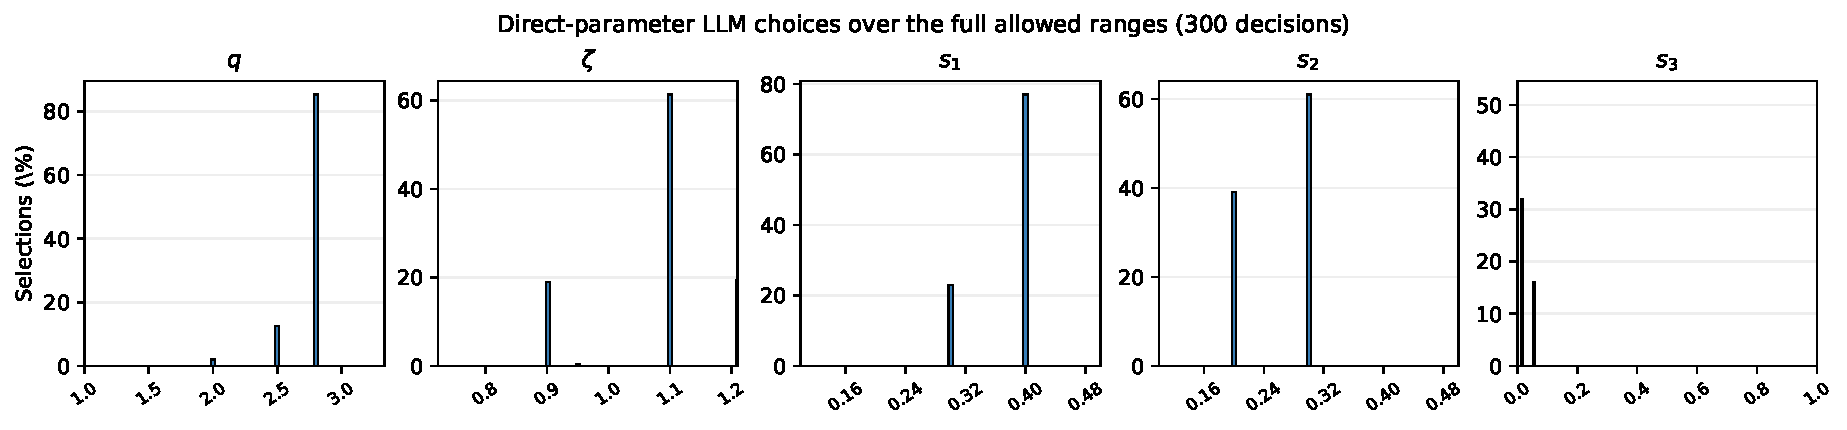
\includegraphics[width=\textwidth]{figures/direct_param_distribution.pdf}
  \caption{Parameter choices aggregated over all six races (300 LLM
  decisions). Bars show discrete selection frequencies after rounding only
  numerical precision.}
  \label{fig:direct-param-distribution}
\end{figure}

Figure~\ref{fig:direct-param-distribution} makes this concentration visible:
$q=2.8$ was selected in 256 of 300 decisions and $s_1=0.4$ in 231. This suggests
that, for this model and prompt, mapping a numerical scene directly to five
coupled MPC parameters is harder than selecting a semantic mode. It does not
show that the manually chosen mode presets are optimal; these can later be
calibrated on a separate scenario set without changing the mode selector or
final test set.

None of the LLM variants met the one-second decision interval. Raw prompts took
approximately 3--4 s, rule prompts 4--5 s, and direct-parameter prompts about
7 s per call. The raw LLM was the strongest preliminary variant, but it also
showed occasional contact or off-road recovery.

These were preliminary results with the earlier shared MPC. The updated
controller results below show that the low-level formulation can change the
relative performance of the high-level policies.

\section{August 18--25, 2026: IBR speed gap and the shared MPC debugging}

\subsection{Why was trajectory IBR much faster than the shared-MPC policies?}

\noindent\textbf{Short answer: trajectory IBR had a more direct action space and
greater speed access; its lead largely disappeared when those advantages were
restricted or removed.}

Trajectory IBR directly optimizes throttle and steering, whereas the LLM and
$\alpha$-RACER select five parameters and rely on the shared MPC. Its initial
advantage was large (Table~\ref{tab:trajectory-ibr-speed}). Restricting IBR
toward the raceline speed removed that advantage, showing that control and speed
access contributed substantially to the result.

\begin{table}[ht]
  \centering
  \small
  \begin{tabular}{lccc}
    \toprule
    Ego policy, 50 s & Wins & Mean progress (m) & Mean speed (m/s) \\
    \midrule
    Trajectory IBR, global limit & 3/3 & 237.3 & 4.74 \\
    Trajectory IBR, raceline-speed bound & 0/3 & 183.0 & 3.61 \\
    Local $\alpha$-RACER self-play & 1/3 & 193.0 & 3.91 \\
    \bottomrule
  \end{tabular}
  \caption{Trajectory-IBR speed-gap screen over three starting positions.}
  \label{tab:trajectory-ibr-speed}
\end{table}

We then implemented Parameter-IBR as a like-for-like diagnostic. It applies
alternating best responses to $(q,\zeta,s_1,s_2,s_3)$ and sends the result
through the same MPC as $\alpha$-RACER and the LLM. In the saved 50 s screen,
its performance was close to the paired $\alpha$-RACER rather than trajectory
IBR (Table~\ref{tab:parameter-ibr-screen}). The Parameter-IBR row pools its two
cars in each race.

\begin{table}[ht]
  \centering
  \small
  \begin{tabular}{lrrr}
    \toprule
    Policy in the paired screen & Samples & Mean progress (m) & Mean speed (m/s) \\
    \midrule
    Parameter-IBR & 6 & 167.2 & 3.42 \\
    Local $\alpha$-RACER & 3 & 174.5 & 3.55 \\
    \bottomrule
  \end{tabular}
  \caption{Parameter-IBR and $\alpha$-RACER using the same five-parameter MPC
  interface.}
  \label{tab:parameter-ibr-screen}
\end{table}

These results motivated an audit of the common raceline and MPC rather than
attributing the original gap entirely to interaction reasoning. The saved data
are under \texttt{result/llm\_baseline\_suite/},
\texttt{result/ibr\_speed\_cap\_suite/}, and
\texttt{result/local\_alpha\_vs\_parameter\_ibr\_corrected/}.
Trajectory IBR is therefore retained as a strong full-trajectory optimization
reference, while Parameter-IBR is retained only as an abstraction-level
diagnostic rather than a primary policy baseline.

\subsection{Did recomputing the raceline improve the local controller?}

\noindent\textbf{Short answer: yes. After correcting the steering calibration,
the regenerated local raceline still increased mean progress in the controlled
screen.}

The released raceline was generated under different vehicle assumptions. A
local minimum-curvature path initially appeared much faster, but this exposed a
historical steering error. Steering is mapped as
\[
  \delta=S_a u_{\mathrm{steer}}+S_b.
\]
The first candidate had been produced with the incorrect historical value
$S_a=0.80$. We restored $S_a=0.34$, $S_b=0$, and wheelbase $0.34\,\mathrm m$,
then regenerated the raceline. Table~\ref{tab:raceline-screen} shows that the
corrected local reference still improved the controlled 15 s screen.

\begin{table}[ht]
  \centering
  \small
  \begin{tabular}{llrr}
    \toprule
    Steering setting & Reference & Three-car progress (m) & Mean (m) \\
    \midrule
    Corrected $S_a=0.34$ & Released
      & $54.12/47.99/40.84$ & 47.65 \\
    Corrected $S_a=0.34$ & Regenerated local
      & $62.43/56.91/51.09$ & 56.81 \\
    \bottomrule
  \end{tabular}
  \caption{Static $15$ s raceline screen after correcting the steering map.}
  \label{tab:raceline-screen}
\end{table}

The corrected screens are stored under
\texttt{result/sa034\_old\_raceline\_screen/} and
\texttt{result/sa034\_new\_raceline\_screen/}. The $S_a=0.80$ candidate is
archived only as diagnostic history.

\subsection{Was the old Cartesian-to-Frenet projection incorrect?}

\noindent\textbf{Short answer: yes. It measured each predicted Cartesian point
in a preselected future reference frame rather than at the point's actual track
projection. The MPC now predicts directly in Frenet coordinates.}

The MPC audit also found a coordinate error. The earlier solver propagated a
symbolic Cartesian prediction $(x_k,y_k)$, but computed its lateral error using
the tangent and normal of the preselected $k$th future reference cross-section.
That is only a local linear approximation to the Frenet projection. When the
predicted vehicle was far from that reference section, the resulting lateral
coordinate could differ substantially from the projection of the predicted
point onto the track.

The shared MPC was therefore rewritten with the internal state
$(s,e,\Delta\psi,v)$. The measured Cartesian state is projected once at the
start of each solve; the optimizer then propagates Frenet dynamics and uses its
predicted $s$ and $e$ directly for tracking, boundary, and collision terms.
After this correction, a 25 s three-car $\alpha$-RACER screen reached
$106.12/109.69/106.27$ m with no boundary violation, recovery, collision, or
failed MPC solve. Parameter-IBR could nevertheless still stall near the same
hairpin, so the projection error was real but was not the sole cause of the
later deadlock. The corresponding checks are retained in
\texttt{result/frenet\_mpc\_alpha\_25s\_w0/} and
\texttt{result/frenet\_mpc\_parameter\_ibr\_deadlock\_recheck\_w05/}.

\subsection{Why could a successful MPC solve still leave the car stopped?}

\noindent\textbf{Short answer: the solver could repeatedly prefer a cheap
near-neutral first action and postpone the acceleration needed to regain
steering authority.}

The corrected setup exposed a repeated failure that the earlier high steering
authority had partly hidden. In a larger comparison, several MPC-based cars
stopped near the same Berlin hairpin at approximately $64$--$65$ m progress.
The NLP solver normally reported a successful solution, so this was not
primarily a solver-crash problem. Figure~\ref{fig:hairpin-stall} shows one 40 s
Parameter-IBR self-play example: two cars stopped at $65.08$ m and $65.55$ m,
while the third continued to $167.01$ m.

\begin{figure}[ht]
  \centering
  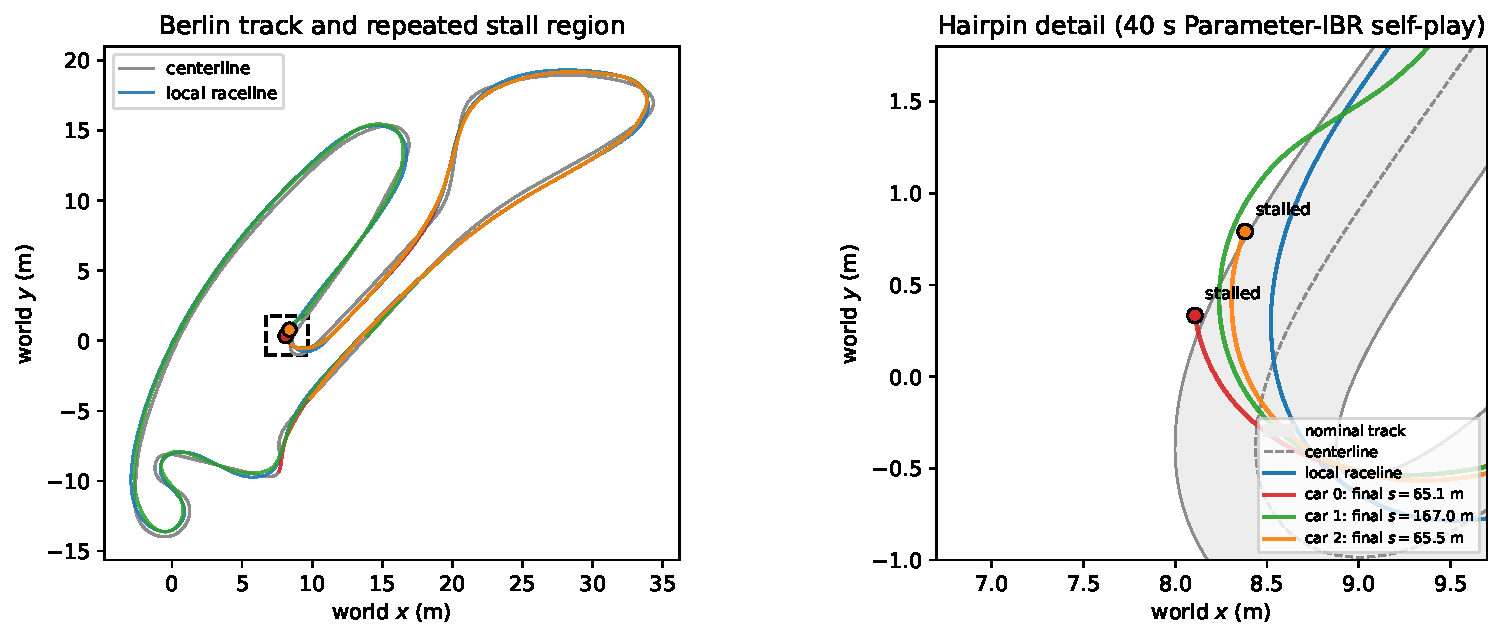
\includegraphics[width=\textwidth]{figures/august23_hairpin_stall.pdf}
  \caption{Repeated low-speed stall near the Berlin hairpin. The left panel
  locates the region on the full track; the right panel shows the local
  raceline, nominal track boundaries, and the three recorded trajectories.}
  \label{fig:hairpin-stall}
\end{figure}

The kinematic yaw rate is proportional to speed, so a nearly stopped car must
accelerate before steering becomes effective. Near the constrained hairpin,
that maneuver can initially increase tracking or slack cost. Receding-horizon
optimization may therefore keep executing a cheap neutral first action while
postponing acceleration. Several alternative penalties, horizons, initial
guesses, and recovery mechanisms were screened, but are retained only in the
development log because none gave a clean general solution.

\subsection{Why did the released project not show the same persistent stall?}

\noindent\textbf{Short answer: its numerical simulator also leaves the track
substantially, but a simulator-level recovery actively redirects the vehicle.}

We also ran the unmodified released $\alpha$-RACER numerical race callback in a
headless wrapper. ROS publishers and visualization messages were replaced by
empty adapters, but the released dynamics, MPC, IBR, checkpoints, initial
states, $0.1$ s update, and 500-step race loop were retained. ROS is therefore
not required for the numerical algorithms themselves.

The released simulator explicitly intervenes after $|e|>0.55$ m by reducing
velocity, rotating the vehicle toward the reference, and adding inward steering.
The following single-race checks show that this recovery is used materially.

\begin{table}[ht]
  \centering
  \small
  \begin{tabular}{lrrr}
    \toprule
    Released setup & Final progress (m) & Maximum $|e|$ (m) & Time $|e|>0.55$ (s) \\
    \midrule
    $\alpha$-RACER vs. MPC vs. MPC
      & $110.4/84.1/117.1$ & $0.867/0.812/0.585$ & $13.3/8.3/1.2$ \\
    $\alpha$-RACER vs. IBR vs. IBR
      & $108.8/120.3/73.5$ & $0.873/0.940/1.315$ & $15.7/10.1/22.3$ \\
    \bottomrule
  \end{tabular}
  \caption{Headless execution of two released 50 s numerical races. Values are
  shown in car order.}
\end{table}

This does not make the local stall desirable, but it changes the interpretation:
the released implementation also does not rely on its MPC or IBR alone to remain
on track. Its simulator-level recovery is an important part of completing a
race. For the local primary comparison, the low-speed recovery supervisor remains
disabled so that policy failures are not silently corrected.

\subsection{Can velocity tracking remove the common MPC stall?}

\noindent\textbf{Short answer: in the controlled hairpin screen, yes. A positive
speed-reference weight changed the outcome from a stationary car to successful
hairpin traversal without changing the solver or adding recovery.}

The shared MPC tracked moving raceline positions but did not explicitly penalize
speed error. We added
\[
  J_v=w_v\sum_{k=0}^{N}(v_k-v_k^{\mathrm{ref}})^2.
\]
It is shared by all five-parameter policies. Table~\ref{tab:velocity-screen}
holds the difficult Position-3 rule-policy screen fixed at $N=10$ and track
slack weight $10^5$. With $w_v=0$ the ego stopped near $64$ m; positive weights
crossed the hairpin, and $w_v=10$ did so without nominal boundary violation.

\begin{table}[ht]
  \centering
  \small
  \begin{tabular}{rrrrr}
    \toprule
    $w_v$ & Progress (m) & Final speed (m/s) & Boundary time (s) & Recovery (s) \\
    \midrule
    0  & 64.2 & 0.00 & 6.06 & 0.00 \\
    1  & 89.1 & 5.00 & 0.34 & 0.00 \\
    3  & 95.2 & 5.00 & 0.20 & 0.00 \\
    10 & 98.0 & 5.00 & 0.00 & 0.00 \\
    \bottomrule
  \end{tabular}
  \caption{Controlled 25 s velocity-tracking screen for the same Position-3
  rule-policy case. All MPC solves succeeded.}
  \label{tab:velocity-screen}
\end{table}

This is evidence that velocity tracking resolved the common low-speed failure
in this screen; it is not proof against every high-level reference. We retained
$N=10$ and the original slack weight rather than making track departures cheap.

\subsection{Did the MPC change generalize across policies and starting positions?}

\noindent\textbf{Short answer: it removed the widespread stall, but raw LLM and
Parameter-IBR each retained one reference-specific failure.}

The table summarizes the updated three-position tests against two locally
trained $\alpha$-RACER cars. ``Stall'' denotes an ego car finishing near zero
speed at the hairpin. Each position was run once, so the table is a regression
check rather than a final statistical evaluation.

\begin{table}[ht]
  \centering
  \small
  \begin{tabular}{lrrrr}
    \toprule
    Ego policy & Wins & Mean progress (m) & Ego stalls & Recovery time (s) \\
    \midrule
    Local $\alpha$-RACER self-play & 1/3 & 99.6 & 0 & 0.00 \\
    Pure rule-based                 & 1/3 & 103.5 & 0 & 0.00 \\
    Raw LLM                         & 0/3 & 86.8 & 1 & 0.22 \\
    Rule-prompt LLM                 & 1/3 & 103.9 & 0 & 0.00 \\
    Parameter-IBR                   & 1/3 & 89.1 & 1 & 0.02 \\
    \bottomrule
  \end{tabular}
  \caption{Updated shared-MPC regression with $N=10$, $w_v=10$, and track-slack
  weight $10^5$.}
\end{table}

\begin{figure}[ht]
  \centering
  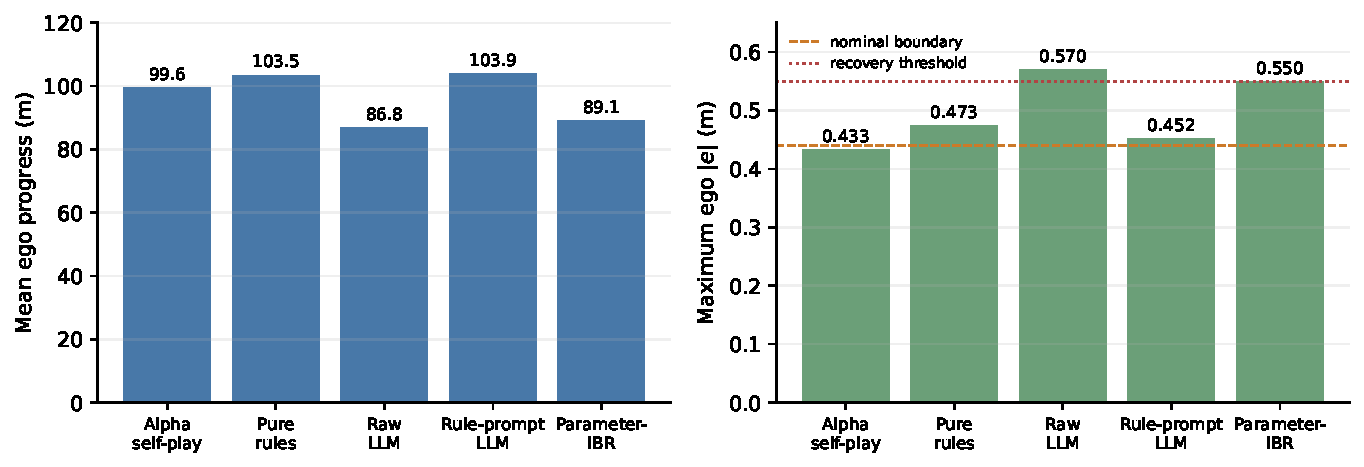
\includegraphics[width=0.96\textwidth]{figures/august25_shared_mpc_comparison.pdf}
  \caption{Mean ego progress and maximum ego lateral error across the three
  starting positions. The dashed and dotted lines mark the local nominal
  boundary and released-simulator recovery threshold.}
  \label{fig:august25-shared-mpc}
\end{figure}

The updated controller removed the earlier widespread stall in $\alpha$-RACER
self-play and in the rule-policy ego runs, without requiring the experimental
terminal or stall-debt penalties. It did not make every high-level reference
recoverable: raw LLM and Parameter-IBR each still produced one hairpin stall.
The remaining failures are therefore treated as outcomes of particular
high-level/reference interactions rather than hidden by another recovery rule.

The policy ordering also changed. The raw LLM selected \emph{push} almost all the
time and stalled from Position 3. The rule-prompt LLM selected mostly
\emph{stable}, completed all three races, and performed similarly to the pure
rule policy. This means the earlier conclusion that explicit rules were simply
too conservative was dependent on the earlier low-level controller. A larger,
held-out comparison is required before making a final prompt claim.

LLM timing remains unresolved. All 75 calls in each prompt condition missed the
one-second decision interval. Raw calls averaged approximately $2.8$ s, while
the longer rule prompt averaged approximately $4.4$ s. The simulator currently
waits for each response, so these tests measure decision quality but not the
physical effect of delayed execution.

The next analysis therefore separated scene understanding from preset quality.
We first checked whether the LLM could extract a simple, verifiable traffic
relationship, without assuming that any one relationship implies a uniquely
correct mode.

\section{August 28--30, 2026: scene understanding and traffic basis}

The next question was whether the raw LLM actually interprets the traffic
observation before selecting a mode. A traffic basis was introduced as a small,
verifiable bridge between numerical observations and tactical decisions. It
describes only an observable relationship; it never prescribes which mode is
correct.

\subsection{Can the traffic basis be checked automatically?}

\noindent\textbf{Short answer: yes. In the retained 45-decision screen, 35
traffic-basis labels were supported, nine were ambiguous, and only one was
contradicted. Among the 36 decisions outside the deadband, factual agreement
was therefore $35/36$ ($97.2\%$).}

For each visible vehicle, let $c$ be its recorded closing speed relative to the
ego car. Positive $c$ means that the gap is shrinking. The evaluator uses the
following rules:

\begin{table}[ht]
  \centering
  \small
  \resizebox{\textwidth}{!}{%
  \begin{tabular}{lll}
    \toprule
    Observation & Front label & Rear label \\
    \midrule
    Vehicle absent
      & \code{no\_front\_vehicle} & \code{no\_rear\_vehicle} \\
    $c>0.1\,\mathrm{m/s}$
      & \code{closing\_on\_front\_vehicle} & \code{rear\_vehicle\_closing} \\
    $c<-0.1\,\mathrm{m/s}$
      & \code{front\_vehicle\_pulling\_away} & \code{rear\_vehicle\_falling\_behind} \\
    $|c|\leq0.1\,\mathrm{m/s}$
      & \code{front\_gap\_approximately\_constant}
      & \code{rear\_gap\_approximately\_constant} \\
    \bottomrule
  \end{tabular}
  }
  \caption{Code-derived traffic-basis criteria. The $0.1\,\mathrm{m/s}$
  deadband is an evaluation convention for nearly constant gaps, not a
  basis-to-mode rule.}
  \label{tab:traffic-basis-rules}
\end{table}

An LLM label is \emph{supported} when it matches the code-derived label. A
dynamic claim is \emph{ambiguous} when $|c|\leq0.1\,\mathrm{m/s}$, and otherwise
a mismatch is \emph{contradicted}. This evaluates
\[
  \text{observation}\longrightarrow\text{traffic basis},
\]
not whether the subsequent mode is tactically optimal.

\begin{figure}[ht]
  \centering
  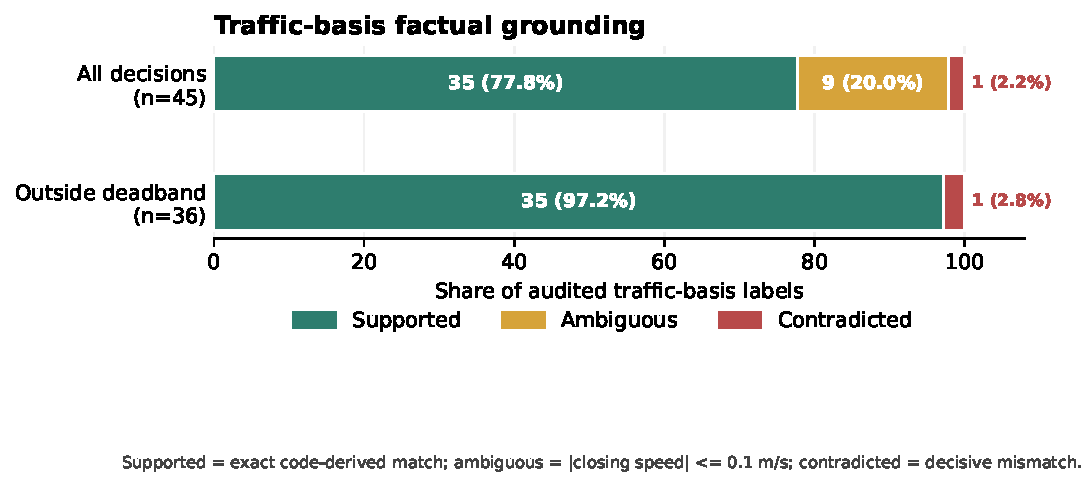
\includegraphics[width=0.88\textwidth]{figures/august30_traffic_basis_grounding.pdf}
  \caption{Factual grounding of the evidence-first traffic basis. The upper
  bar reports all 45 decisions. The lower bar excludes the nine measurements
  inside the closing-speed deadband; it is the appropriate comparison for
  claims that can be judged decisively.}
  \label{fig:traffic-basis-grounding}
\end{figure}

\subsection{Does generating a traffic basis change the online policy?}

\noindent\textbf{Short answer: the LLM usually described the traffic correctly,
but that information did not change its online action in this screen. Both
policies selected \emph{push} throughout and produced the same race result.}

The two one-call policies differ only in generation order:

\begin{figure}[ht]
  \centering
  \setlength{\fboxsep}{7pt}
  \small
  \resizebox{\textwidth}{!}{%
  \begin{tabular}{c@{\quad$\longrightarrow$\quad}c@{\quad$\longrightarrow$\quad}c}
    \fbox{\strut Numerical observation}
      & \fbox{\strut Raw LLM: mode $\rightarrow$ free basis}
      & \fbox{\strut Mode + basis + reason} \\[1.2em]
    \fbox{\strut Numerical observation}
      & \fbox{\strut Evidence-first: traffic basis $\rightarrow$ mode}
      & \fbox{\strut Basis + mode + reason}
  \end{tabular}
  }
  \caption{Raw and evidence-first online decision flows. The evidence-first
  output is autoregressive: its mode is generated after its traffic basis in
  the same LLM call.}
  \label{fig:raw-evidence-flow}
\end{figure}

The controlled screen used three 15 s Berlin races, one from each ego starting
position, against two local $\alpha$-RACER cars. Both policies used the same
observation, model, mode presets, MPC, and temperature.

The grounding result in Figure~\ref{fig:traffic-basis-grounding} shows that the
new intermediate representation was meaningful: the LLM could usually extract
a correct traffic relationship from the observation. However, both raw and
evidence-first policies selected \emph{push} in all 45 decisions. Each won one
of three races and their mean progress was the same to the reported precision
($61.25\,\mathrm{m}$). The unchanged race result is therefore secondary: the
important diagnosis is that factual observation-to-basis grounding succeeded,
whereas the online basis-to-mode response collapsed to one action. A separate
development test also requested a track basis, but only $5/45$ track labels
were supported; that extra task was removed from the retained pipeline.

\subsection{Does the basis actually influence mode selection?}

\noindent\textbf{Short answer: yes in the offline probe, especially for rear
traffic, but the probe measures sensitivity rather than mode accuracy or race
performance.}

The online experiment could not isolate the basis because observation, basis,
and mode were processed in one call. The offline probe adds three controls: the
observation is frozen, the basis is supplied rather than generated inside the
decision call, and only the mode is newly generated. The \emph{generated}
condition first tests whether this separation alone changes the output; the
\emph{oracle} condition removes factual basis error or subject-selection
ambiguity; and the reversed condition tests sensitivity to the relationship
itself. We sampled 11 saved observations and supplied one of three labels:

\begin{itemize}
  \item \emph{generated}: the label previously produced by the LLM;
  \item \emph{oracle}: the factual label computed from
  Table~\ref{tab:traffic-basis-rules};
  \item \emph{counterfactual}: the oracle relation reversed, for example
  \code{rear\_vehicle\_closing} changed to
  \code{rear\_vehicle\_falling\_behind}.
\end{itemize}

Here ``oracle'' means only that the traffic statement is correct. It does not
provide an oracle mode and does not assume a hand-written policy is optimal.
The additional control compared with the online experiment is illustrated in
Figure~\ref{fig:oracle-probe-flow}.

\begin{figure}[ht]
  \centering
  \setlength{\fboxsep}{7pt}
  \small
  \resizebox{\textwidth}{!}{%
  \begin{tabular}{c@{\quad$+$\quad}c@{\quad$\longrightarrow$\quad}c}
    \fbox{\strut Same frozen observation}
      & \fbox{\strut Generated / oracle / reversed basis}
      & \fbox{\strut Fresh mode-only LLM call}
  \end{tabular}
  }
  \caption{Offline intervention used to isolate the effect of the supplied
  traffic relationship on mode selection. No selected mode was executed.}
  \label{fig:oracle-probe-flow}
\end{figure}

\begin{figure}[ht]
  \centering
  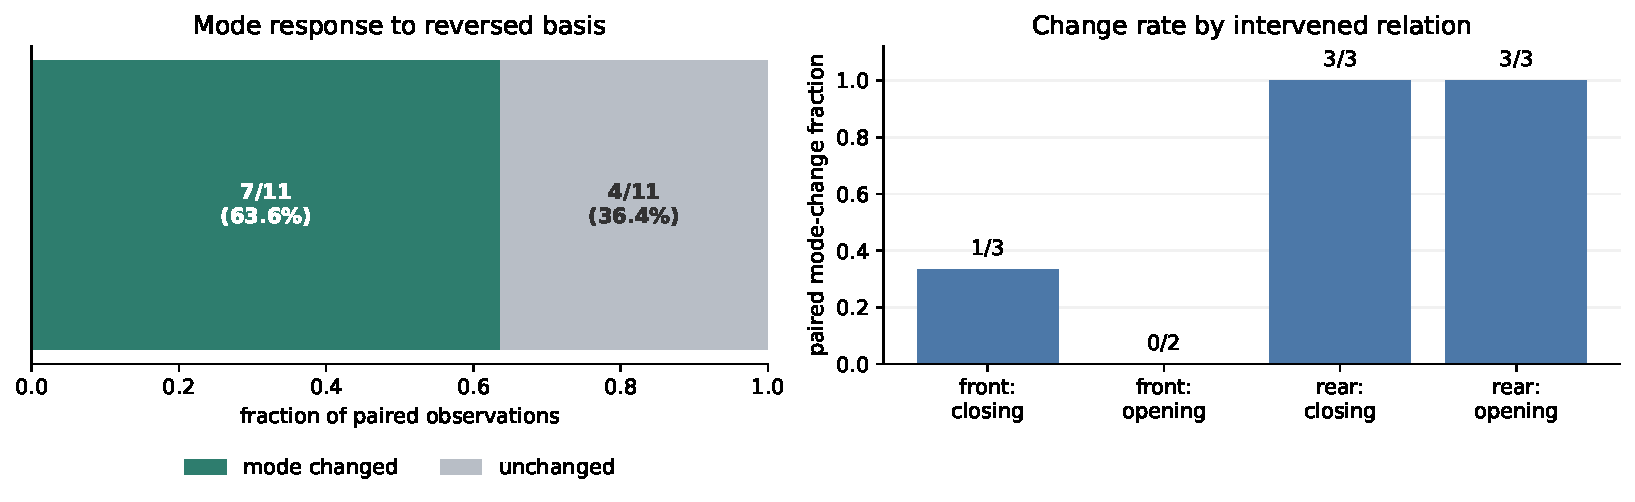
\includegraphics[width=0.96\textwidth]{figures/august30_basis_intervention.pdf}
  \caption{Paired sensitivity to the supplied traffic basis. Each comparison
  keeps the saved observation fixed and reverses only its oracle traffic
  relation. The bars report whether the newly selected mode changes for that
  same observation, rather than comparing aggregate mode counts.}
  \label{fig:basis-intervention-change-rate}
\end{figure}

Changing the oracle basis to its reversed counterpart changed the selected mode
in $7/11$ paired cases ($63.6\%$). Sensitivity was strongest for rear traffic:
all three rear-closing and all three rear-opening interventions changed the
mode. Only one of three front-closing interventions and neither of the two
front-opening interventions did so. The earlier aggregate mode counts are not
used as the main sensitivity measure because different paired changes can
cancel in the overall distribution.

The experiment therefore shows that a supplied traffic relation can affect the
LLM's mode, and that separating relation extraction from mode selection reduces
the all-push distribution in this small probe. It does \emph{not} establish that
the new modes are correct: no unique ground-truth mode was defined and none of
the offline actions was executed. In addition, this first probe holds the
numerical observation fixed while reversing its basis, so it is an input-conflict
sensitivity test rather than a physically consistent counterfactual scene.
Evaluating basis-to-mode quality will require paired, internally consistent
observation changes and counterfactual rollouts under fixed mode presets.

\end{document}
